\section{Objekt Orientiertes Programmieren - OOP}
Wie jede OOP Sprache unterstützt auch Java das Konstrukt der Klassen, Vererbung und Polymorphismus. Eine \textbf{Klasse} ist eine Art Bauplan, hingegen ein \textbf{Objekt} die erstellten Gebäude ansich sind. Die \textbf{Instanz} ist ein einzigartiges Objekt, in diesem Fall ein spezifisches Gebäude. Instanzen werden mit dem Operator \textit{new} erstellt.
\begin{lstlisting}
	Buildung b = new Buildung();
\end{lstlisting}
Wichtig ist, dass jedes Objekt in Java vom Basisobjekt \textit{Object} erbt. Desshalb sind auf allen Instanzen folgende Methoden verfügbar:
\begin{itemize}[nosep]
	\item public String toString()
	\item public boolean equals(Object obj)
	\item public int hashCode()
\end{itemize}

\subsection{Methoden}
Methoden können in Klassen definiert werden. Diese Methode ist jedoch an das Objekt gebunden und kann Instanzvariablen modifizieren. Ausser Methode oder Instanzevariable ist mit \textit{static} deklariert.

Duch Generics (1) können auch einzelne Methoden verallgemeinert werden. Falls eine offene Anzahl an Parametern benötigt wird, können Varargs (2) eingesetzt werden.
\begin{lstlisting}
// (1)
public <E> Stack<E> getStack(E value, int times) { }
public <E> void push(E... items) { }
\end{lstlisting}


\subsection{Vererbung}
Java unterstützt die Vererbung mittels den Keywords \textit{extends} und \textit{implements} für Interfaces.\\
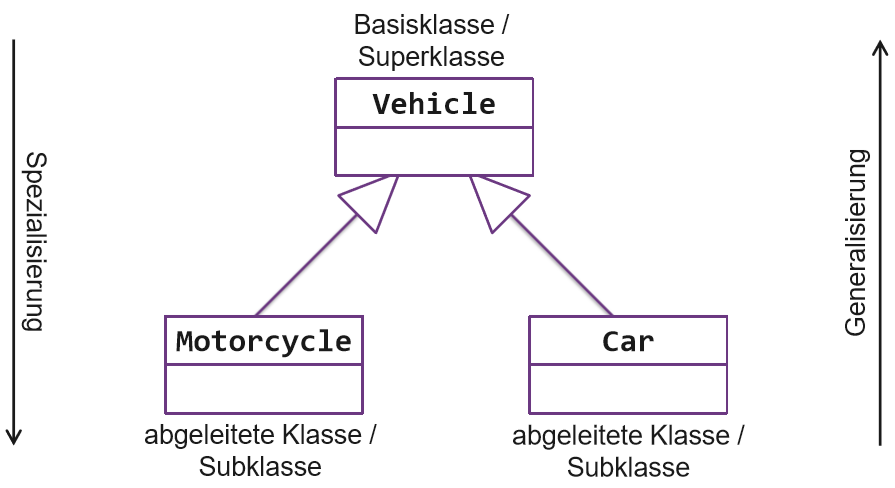
\includegraphics[width=\columnwidth]{Images/vererbung}

Die Vererbung kann durch Generics eingeschränkt werden
\begin{lstlisting}
class GraphicStack<T extends Graphic> extends Stack<T> {
	...
}
\end{lstlisting}


\subsection{Overloading}
Das Konzept von overloading beschreibt die Möglichkeit Methoden zur Laufzeit (dynamisch) zu überschreiben. Wenn abstract verwendet wird, kann der Kompiler die Methode bereits statisch evaluieren.

\begin{lstlisting}
	public class Programm {
		public static void main(String args[]) {
			Car c = new Car();
			Vehicle v =  c;
			v.print();	// prints: Car
			c.print();  // prints: Car
			
			v = new Vehicle();
			v.print();	// prints: Vehicle
		}
	}
	
	class Vehicle {
		public String getKind () {
			return "Vehicle";
		}
		
		public void print() {
			System.out.println(getKind());
		}
	}
	
	class Car extends Vehicle {
		@Override
		public String getKind() {
			return "Car";
		}	
	}
\end{lstlisting}

\textbf{Wichtig:} Attribut \textit{@Override} ist freiwillig, der Kompiler weist jedoch bei Fehlender Basis Method auf einen Fehler hin.